\section{Choosing Comparison Units}

\begin{frame}{Motivation}
Let us decompose the treatment effect $\tau$. \\
\vspace{5pt}
\begin{itemize}
    \item $Y_{it}^{(1)}$: The set of treated outcomes is observed. Assuming the absence of measurement error, the data are accurate. 
    \vspace{-7pt}
    \item $Y_{it}^{(0)}$: The set of untreated potential outcomes are not observed. Bias and inaccuracies likely stem from (i) prediction errors of the untreated data but also (ii) the choice of untreated units we choose to compare our observed treated unit with.
\end{itemize}

Therefore, even if we have generated reliable synthetic data for the untreated outcomes, that leaves us with one important choice:\\ 
\vspace{5pt}
\centering
\textbf{Which control units $Y_{it}^{(0)}$ do we compare our treated unit $Y_{it}^{(1)}$ with to obtain $\tau$?}
\end{frame}

\begin{frame}{Context}
Intuitively, this problem equates to not wanting to compare apples to oranges. \\
\vspace{5pt}
\begin{enumerate}
    \item Using a set of covariates $X_{it}$ to control for confounders (Pollmann WP)
        \begin{itemize}
            \item Pros: It is easy to overlay spatial distributions of covariates in a map (Think: Each covariate is a separate heatmap)
            \item Cons: Curse of dimensionality; does not capture unobserved heterogeneity
        \end{itemize}
    \item Using the k nearest units as comparison units
        \begin{itemize}
            \item Pros: It is easy to implement and intuitive
            \item Cons: Disregards more complex spatial relationships; breaks in higher dimensions; inherently arbitrary
        \end{itemize}
    \item Using spatial first differences (Druckenmiller \& Hsiang, 2019)
        \begin{itemize}
            \item Pros: It does account for unobserved heterogeneity (Think: Mini RDs between spatially adjacent units); No functional form assumptions and purely data-driven
            \item Cons: Breaks in higher dimensions
        \end{itemize}
\end{enumerate}
\end{frame}

\begin{frame}{The Spatial First Differences Idea}

Spatial first differences do remove unobserved heterogeneity, great!\\
\vspace{5pt}
\centering
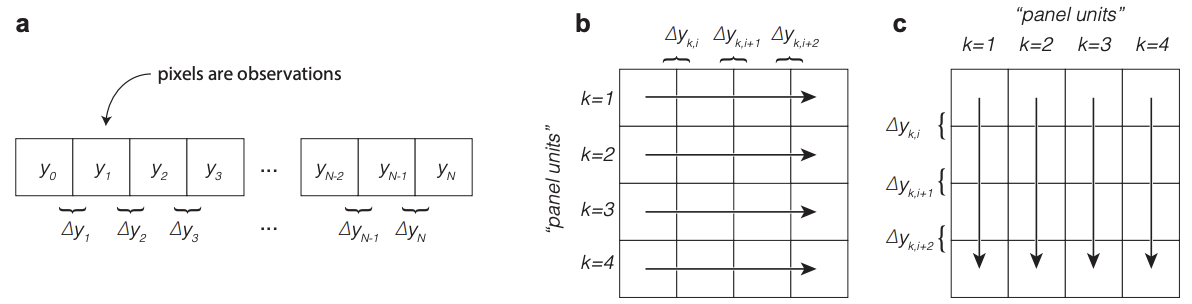
\includegraphics[scale=0.67]{figures/spatialfd.png}
\caption{\footnotesize{Druckenmiller \& Hsiang, 2018}}\\
\vspace{7pt}
\Rightarrow \textbf{ However, this approach breaks down when we want to account for a (non-pooled) time dimension. Can we borrow any ML tools to deal with this high-dimensional problem?}
\end{frame}

\begin{frame}{A Geometric Learning Approach}

\begin{columns}
% Split 1
\begin{column}{0.45\linewidth}
\begin{itemize}
    \item Let us consider a graph where the nodes correspond to the units, and the edges between them represent the spatial differences. 
    \vspace{-7pt}
    \item Then, the length of the edges can be a measure of the similarity of units under identical treatment status. 
    \vspace{-7pt}
    \item When adding the time dimension, the graph consists of both spatial and temporal edges.
\end{itemize}
\end{column}
% Split 2
\begin{column}{0.6\linewidth}
\centering
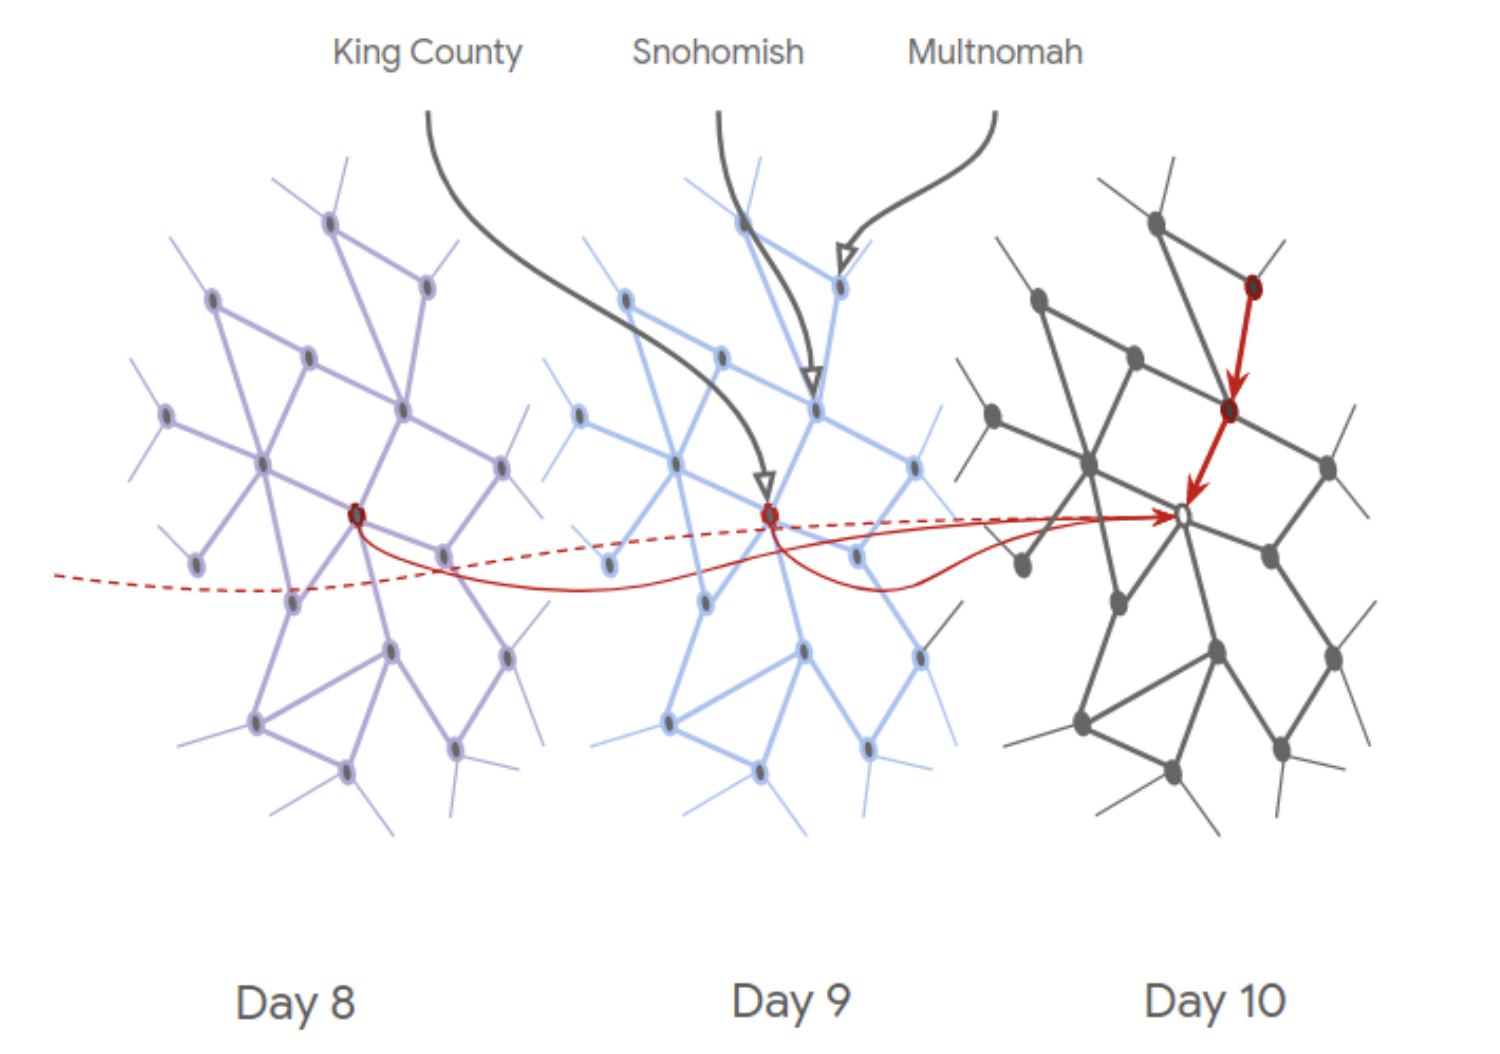
\includegraphics[scale=0.33]{figures/gnn.png}
\caption{\footnotesize{Kapoor, Ben et al., 2020: COVID-19 Infections}}
\end{column}
\end{columns}
\end{frame}

\begin{frame}{A Geometric Learning Approach (ctd.)}

As long as we do not compare units across treatment status, we will obtain a three-dimensional graph. The edges represent a measure of similarity - a spatial or temporal first difference, respectively that is standardized across dimensions.\\
\vspace{3pt}
\begin{columns}
    \begin{column}{0.85\linewidth}
    Formally, we can use a graph clustering algorithm to divide this 3-D graph into subsets. These k subsets will:
    \begin{itemize}
        \item Be between 1 < k < n, where 1 would include all units and n will construct a separate cluster for each unit in space and time
        \vspace{-7pt}
        \item Minimize the within-cluster average edge length: $\bar{E} = \frac{1}{k}\sum_{it}^{IT}(E)$; $\forall i \in I, t \in T.$
        \item Note: The spatial dimension shall be finely gridded. Coarse grids may omit valuable information. 
    \end{itemize}
    \end{column}
    % Split 2
    \begin{column}{0.17\linewidth}
        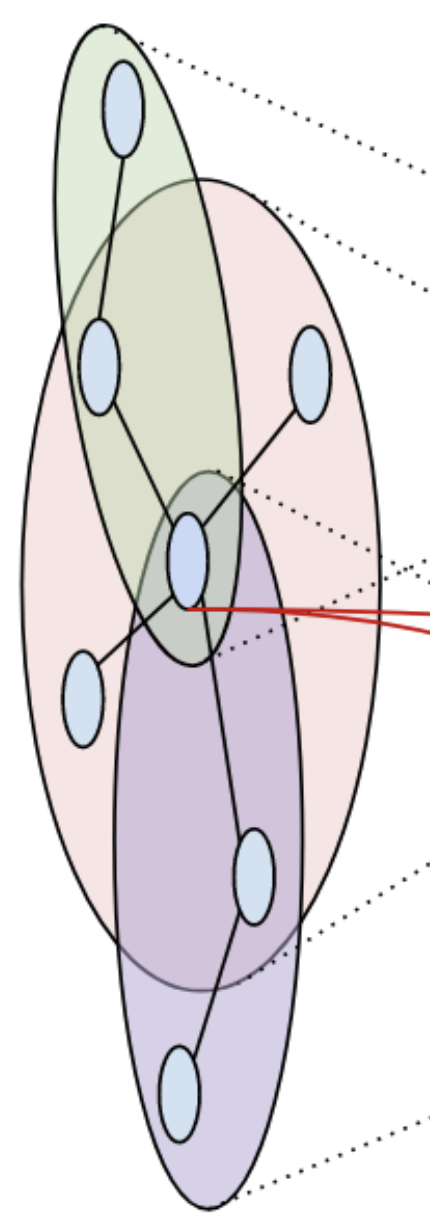
\includegraphics[scale=0.21]{figures/gnn_cluster.png}
        \caption{}
    \end{column}
\end{columns}
\end{frame}

\begin{frame}{Outcome and Practical Challenges}

The desired outcome is a set of k clusters within which all units are comparable across space and time. Metaphorically, we are sorting a basket of apples and oranges into two separate baskets containing apples and oranges, respectively. 

Notably, there are considerable implementation challenges:\\
\begin{itemize}
    \item As $k \rightarrow n$, $\bar{E}$ may monotonically decrease s.t. there is no $k$ that minimizes $\bar{E}$ other than $k=n$
    \vspace{-7pt}
    \item Approaches to finding this optimal k have included the elbow and silhouette methods
    \vspace{-7pt}
    \item Optimization literature may give insight into appropriate constraints, e.g., continuity, non-separability, and overlap of clusters. 
\end{itemize}
\end{frame}
